\section{Gnomio}


\begin{figure}
\centering
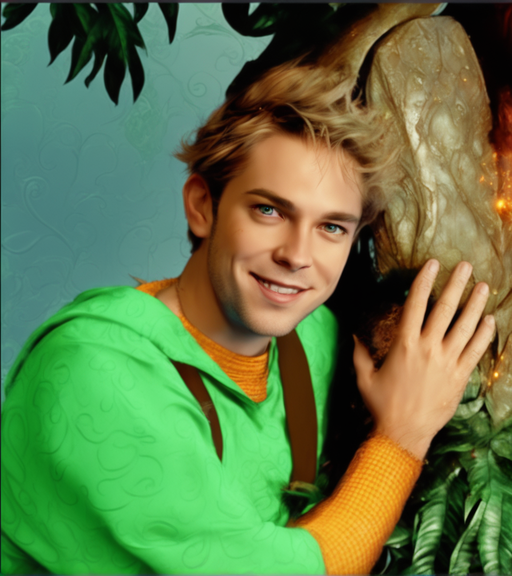
\includegraphics{gnomo-epic-royal-background-big-royal-uncropped-crown-royal-jewelry-robotic-nature-full-shot-.png}
\caption{gnomo-epic-royal-background-big-royal-uncropped-crown-royal-jewelry-robotic-nature-full-shot-.png}
\end{figure}

Informazioni Generali

Età:

Data di nascita:

Luogo di nascita:

Razza:

Classe:

Alleati:

Nemesi:

Alias:

Professione:


\subsection{1. Descrizione Generale}\label{descrizione-generale}


\begin{figure}
\centering
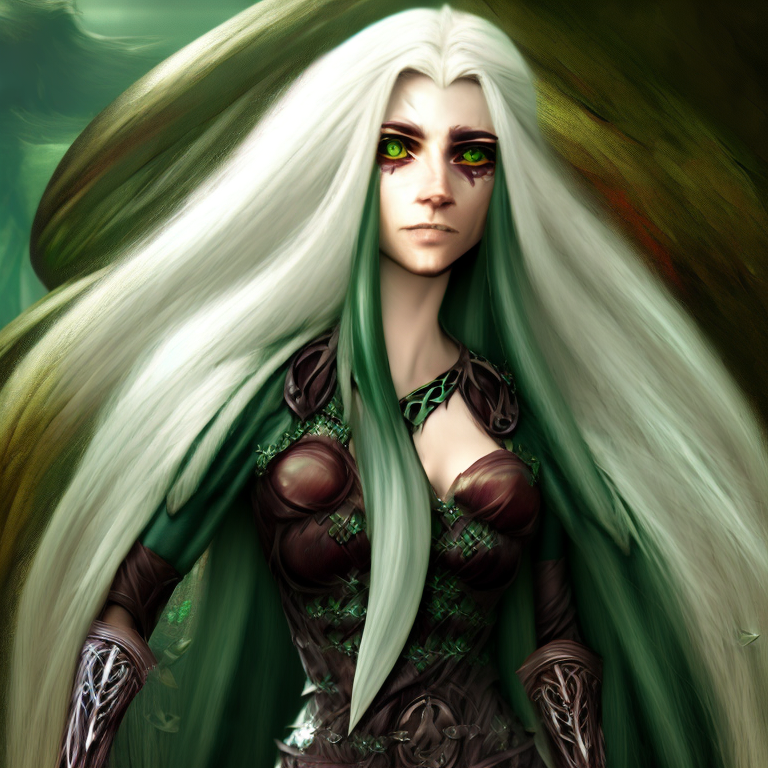
\includegraphics{full-body-portrait-of-a-beautiful-female-elf-with-long-silver-hairs-and-deep-green-eyes-fantasy-se-.png}
\caption{full-body-portrait-of-a-beautiful-female-elf-with-long-silver-hairs-and-deep-green-eyes-fantasy-se-.png}
\end{figure}

Gnomio è uno gnomo giovane e intraprendente che vive nel tranquillo
Fantabosco, un affascinante villaggio gnomico situato nella Valtara
Meridionale, al confine con il Regno degli Alisei. Sin da bambino, ha
sognato di diventare uno dei più grandi eroi di Fantabosco e ha un
desiderio ardente: uccidere un drago e creare un'armatura di scaglie di
drago che diventi leggendaria a Valtara. La sua vita è un'avventura in
continua evoluzione, guidata dalla passione per la storia dei draghi e
il desiderio di gloria.

\begin{quote}
``Che testa di pigna che sono!''
\end{quote}

\subsection{2. Biografia}\label{biografia}


Gnomio è nato a Fantabosco da una famiglia di gnomi con una lunga
tradizione di artigianato. Fin dall'infanzia, è stato affascinato dalle
storie dei draghi raccontate dai viaggiatori che passavano per il suo
villaggio. La madre di Gnomio, Mamma Antelitteram, è stata una figura
determinante nella sua vita, spingendolo ad avvicinarsi alla Gilda dei
Protettori per poter garantire il suo sostentamento. Questo è stato un
passo cruciale che ha influenzato la sua carriera.

\subsection{3. Carriera}\label{carriera}


La passione di Gnomio per la storia dei draghi lo ha spinto a diventare
un abile archeologo, dedicando innumerevoli ore a scavare tra le rovine
antiche e a esaminare manufatti per apprendere tutto ciò che poteva. Da
adulto, ha deciso di diventare un ranger specializzato nella caccia alle
creature magiche, in particolare ai draghi. Ha perfezionato le sue
abilità di combattimento, apprendendo a sopravvivere nella natura
selvaggia e ad affrontare i pericoli della Foresta dei Giganti.

Il suo percorso lo ha portato a viaggiare in luoghi remoti alla ricerca
di indizi sulle possibili dimore dei draghi. L'affiliazione alla Gilda
